\pagestyle{circuito}
\label{circuito}

\begin{textblock*}{5.625in}(0pt,0pt)%
\vspace*{-1.45cm}
\hspace*{-1.8cm}\includegraphics*[width=112mm]{./imgs/CIRCUITO.png}
\end{textblock*}

\pagebreak

\hspace{.5cm}

\begin{center}
\hspace*{-1cm}\raisebox{5.5cm}{\rotatebox[origin=t]{90}{\Formular{\textbf{Lançamento}}}}
\hspace{1cm}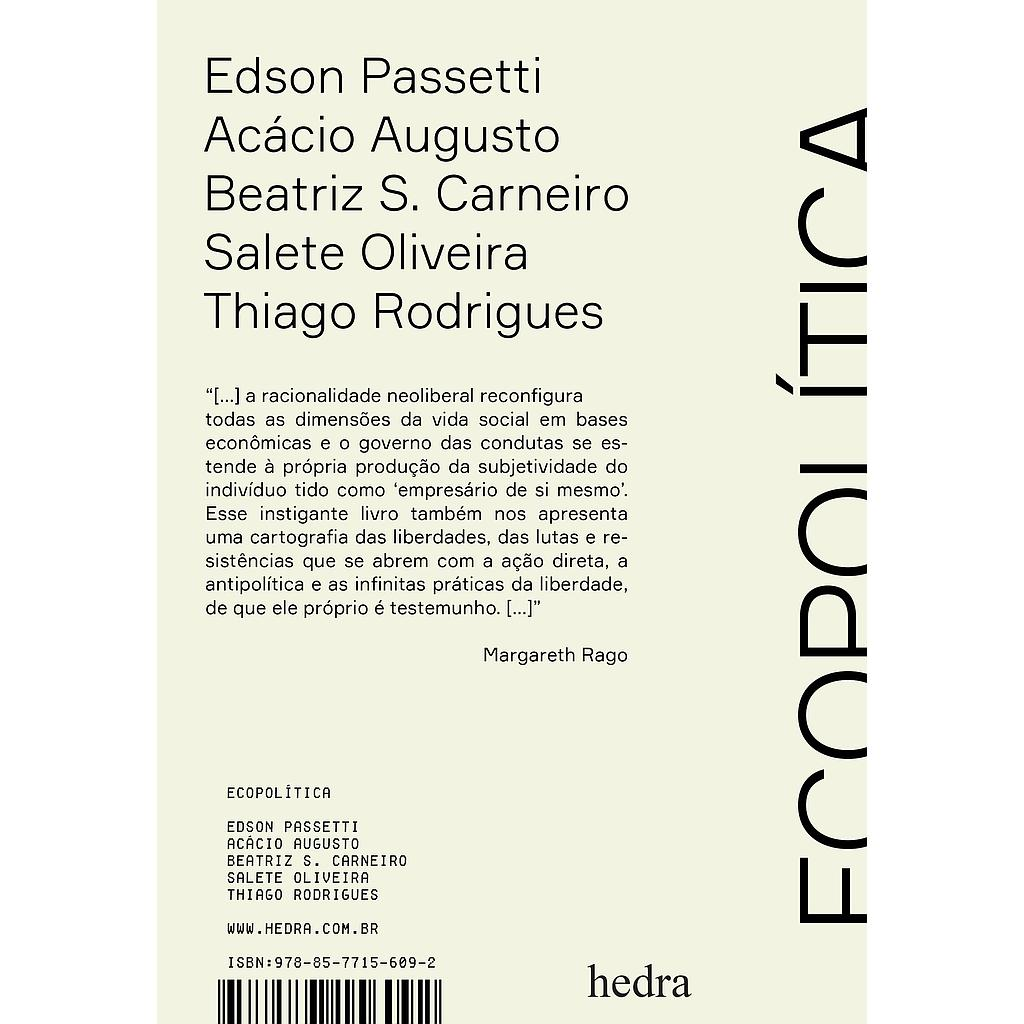
\includegraphics[width=70mm]{eco.jpeg}
\end{center}

\hspace*{-2cm}\_\_\_\_\_\_\_\_\_\_\_\_\_\_\_\_\_\_\_\_\_\_\_\_\_\_\_\_\_\_\_\_\_\_\_\_\_\_\_\_\_\_\_\_\_\_\_\_\_\_\_\_\_\_\_\_\_\_\_\_\_\_\_\_\_\_\_\_\_\_\_\_\_\_

\medskip

\noindent{}Essa obra questiona a noção de origem, original, único, essência originária. Afinal, o que afirmamos quando dizemos que algo é original? Desde Aristóteles já sabemos que a imitação – ou mímesis – deveria recriar a potência de vida e não sua forma. É com base nesse pensamento que o autor pode afirmar que o cover cria {\slsc{COM}} sua base precedente e, sem qualquer hierarquia preestabelecida, inventa outro original.

\hspace{.5cm}

\hspace*{-.4cm}\begin{minipage}[c]{0.90\linewidth}
\small{
{\Formular{\textbf{
\hspace*{-.1cm}Título: As artes do cover\\
Autor: Henrique Saidel\\ 
Editora: Circuito\\
Páginas: 352\\
Formato: 14x21cm\\
Preço: R\$ 55,00\\
ISBN: 978-85-9582-049-4
}}}}
\end{minipage}

\pagebreak

\hspace{.5cm}

\begin{center}
\hspace*{-.5cm}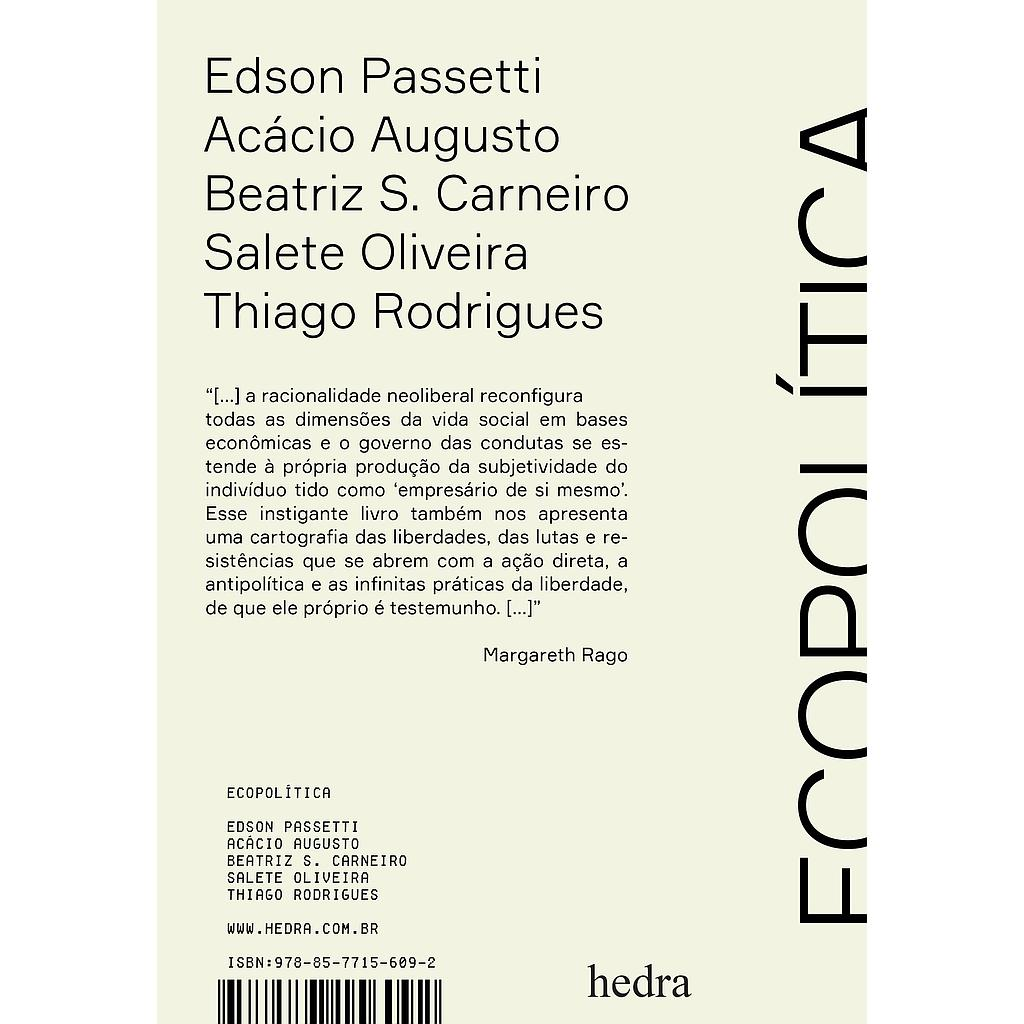
\includegraphics[width=70mm]{eco.jpeg}
%\hspace*{6cm}\raisebox{2cm}{\rotatebox[origin=t]{90}{\Formular{\textbf{Lançamento}}}}
\end{center}

\hspace*{-2cm}\_\_\_\_\_\_\_\_\_\_\_\_\_\_\_\_\_\_\_\_\_\_\_\_\_\_\_\_\_\_\_\_\_\_\_\_\_\_\_\_\_\_\_\_\_\_\_\_\_\_\_\_\_\_\_\_\_\_\_\_\_\_\_\_\_\_\_\_\_\_\_\_\_\_

\medskip

\noindent{}Glossário ilustrado de cidades visitadas pelo artista, pequenas histórias e ilustrações de Alex Cerveny. Prefácio de Renato Rezende, posfácio de Rodrigo Petronio.

\hspace{.5cm}

\hspace*{-.4cm}\begin{minipage}[c]{0.90\linewidth}
\small{
{\Formular{\textbf{
\hspace*{-.1cm}Título: Todos os lugares\\
Autor: Alex Cerveny\\ 
Editora: Circuito\\
Páginas: 190\\
Formato: 16x23cm\\
Preço: R\$ 80,00\\
ISBN: 978-85-9582-050-0
}}}}
\end{minipage}

\pagebreak

\hspace{.5cm}

\begin{center}
\hspace*{-2.5cm}\raisebox{5.5cm}{\rotatebox[origin=t]{90}{\Formular{\textbf{Lançamento}}}}
\hspace{2cm}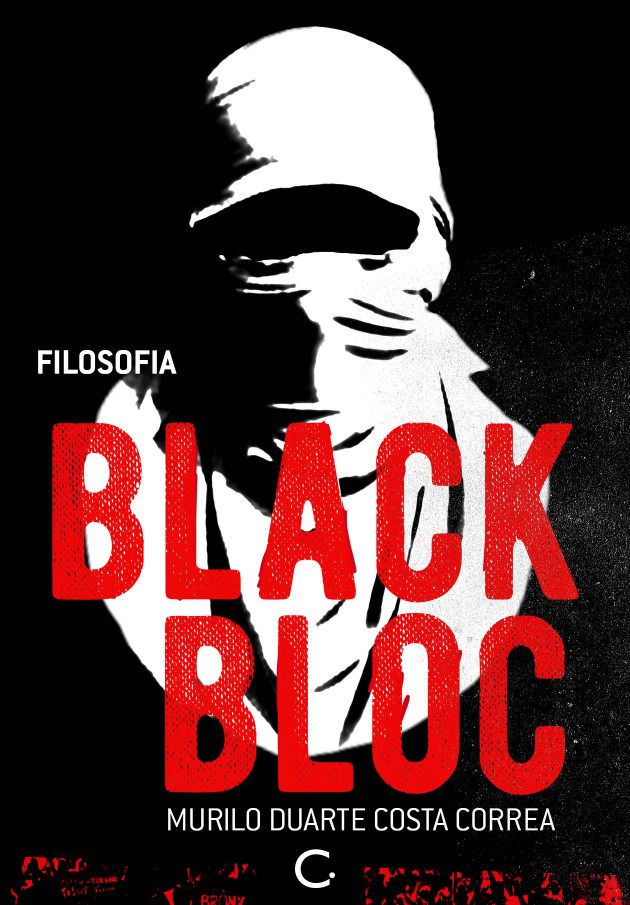
\includegraphics[width=45mm]{./imgs/blackbloc.jpg}
\end{center}

\hspace*{-2cm}\_\_\_\_\_\_\_\_\_\_\_\_\_\_\_\_\_\_\_\_\_\_\_\_\_\_\_\_\_\_\_\_\_\_\_\_\_\_\_\_\_\_\_\_\_\_\_\_\_\_\_\_\_\_\_\_\_\_\_\_\_\_\_\_\_\_\_\_\_\_\_\_\_\_

\medskip

\noindent{}Em junho de 2013, na maior erupção social recente, o Black bloc ganhou os holofotes como nova prática de luta. Analistas foram forçados a compreendê-lo, normalmente municiando um repertório conceitual que não entendia o Black bloc em seus próprios termos. {\slsc{Filosofia Black bloc}} procura suprir essa carência e conceber um arcabouço teórico que permita abordar o Black bloc como fenômeno. Produzir, no pensamento, uma filosofia Black bloc.

\hspace{.5cm}

\hspace*{-.4cm}\begin{minipage}[c]{0.45\linewidth}
\small{
{\Formular{\textbf{
\hspace*{-.1cm}Título: Filosofia Black bloc\\
Autor: Murilo D. C. Correa\\ 
Editora: Circuito\\
Páginas: 166\\
Formato: 12,7x19,1cm\\
Preço: R\$ 46,90\\
ISBN: 978-85-9582-056-2
}}}}
\end{minipage}

\pagebreak

\hspace{.5cm}

\begin{center}
\hspace*{-.5cm}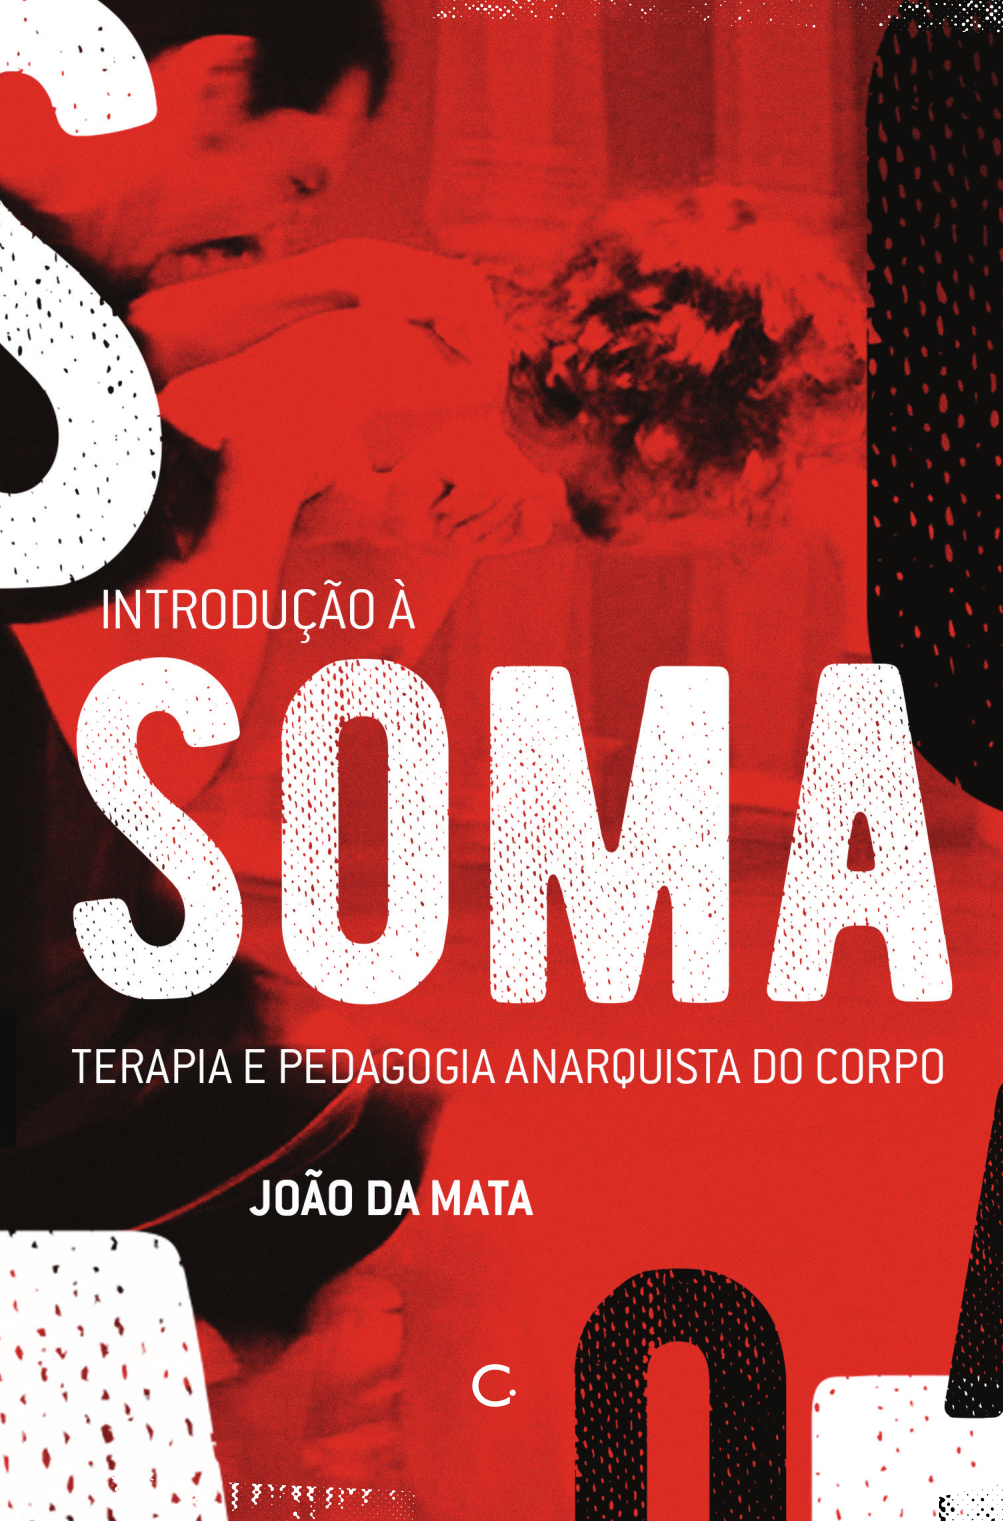
\includegraphics[width=45mm]{./imgs/soma.jpg}
%\hspace*{6cm}\raisebox{2cm}{\rotatebox[origin=t]{90}{\Formular{\textbf{Lançamento}}}}
\end{center}

\hspace*{-2cm}\_\_\_\_\_\_\_\_\_\_\_\_\_\_\_\_\_\_\_\_\_\_\_\_\_\_\_\_\_\_\_\_\_\_\_\_\_\_\_\_\_\_\_\_\_\_\_\_\_\_\_\_\_\_\_\_\_\_\_\_\_\_\_\_\_\_\_\_\_\_\_\_\_\_

\medskip

\noindent{}{\slsc{Introdução à \scalebox{.8}{SOMA}}} trata de um processo terapêutico realizado em grupo, corporal, que busca no pensamento anarquista uma crítica às formas de poder impregnadas no comportamento individual. O grupo funciona como um micro"-laboratório social, daí sua originalidade: a terapia é criação de si, em que a construção das práticas de liberdade é o antídoto para os conflitos gerados pelas hierarquias sociais.

\hspace{.5cm}

\hspace*{-.4cm}\begin{minipage}[c]{0.9\linewidth}
\small{
{\Formular{\textbf{
\hspace*{-.1cm}Título: Introdução à \scalebox{.8}{SOMA}: terapia e pedagogia anarquista do corpo\\
Autor: João da Mata\\ 
Editora: Circuito\\
Páginas: 106\\
Formato: 12,7x19,1cm\\
Preço: R\$ 42,90\\
ISBN: 978-85-9582-055-5
}}}}
\end{minipage}

\pagebreak
